\documentclass{article}
\usepackage{graphicx} % Required for inserting images
\usepackage{authblk}
\usepackage{cite}
\usepackage{natbib}
\usepackage{dcolumn}
\usepackage{pdfpages}
\usepackage{epigraph} % Required for inspirational quote
% packages required for kable()
\usepackage{booktabs}
\usepackage{longtable}
\usepackage{array}
\usepackage{multirow}
\usepackage{wrapfig}
\usepackage{float}
\usepackage{colortbl}
\usepackage{pdflscape}
\usepackage{tabu}
\usepackage{threeparttable}
\usepackage{threeparttablex}
\usepackage[normalem]{ulem}
\usepackage{makecell}
\usepackage{xcolor}
\renewcommand{\epigraphsize}{\small}
\setlength{\epigraphwidth}{0.51\textwidth}
\renewcommand{\textflush}{flushright}
\renewcommand{\sourceflush}{flushright}


%\date{Draft -- please do not circulate.}

\title{(In)civility on Display: Social Media Discourse through the Ideological Lens}

\author[1]{David Broska}
%\author[2]{Byungkyu Lee}
%\author[3]{Barum Park}
%\author[4]{Daniel A. McFarland}
%\affil[1,4]{Stanford University}
%\affil[2]{New York University}
%\affil[2]{Cornell University}

\begin{document}

\maketitle

\epigraph{Civility costs nothing and buys everything.}{Mary Wortley Montagu 1756}
\epigraph{Civility is on the ballot.}{Barack Obama 2016}
%Respect for women is on the ballot. Tolerance is on the ballot. Justice is on the ballot. Equality is on the ballot. Democracy is on the ballot.

\section{Introduction}

Conversations are at the heart of democracies. Discussions in parliaments, media, and kitchen tables inform the political process, help identify solutions to problems, avoid violent conflict, and foster a better understanding of each other. Some consider conversations based on reason rather than content and ignorance even a benchmark for achieving a democracy \citep{sanders_against_1997}. Attaining these outcomes requires \textit{civility} from the interlocutors because it sets the stage for productive conversations. 
At a minimum,  civility means ``demonstrating mutual respect" \citep{mutz_inyourface_2016} or ``politeness" \citep{frimer_montagu_2018}. A maximalist definition of civility does not only require being respectful and polite but also critical engagement \citep{kant_enlightenment_1784}\footnote{Kant does not only argue that individuals should not only have the freedom but also the courage to make use of their own understanding -- i.e., to actively engage. For example, the clergyman is required to teach lessons aligned with the ``creed of the church he serves, for he was employed by it on that condition. But as a scholar he has complete freedom and is even called upon to communicate to the public all his carefully examined and well-intentioned thoughts about what is erroneous in that creed and his suggestions for a better arrangement of the religious and ecclesiastical body."} and requires individuals to give rationales in conversation \citep{habermas1985theory}. In other words, this expanded definition of civility demands contributions to conversations to be productive above and beyond avoiding offense.

While this distinction is grounded in venerable theoretical traditions, it remains unclear how these perspectives align with the public's perception of desirable norms in conversations. Civility is a \textit{social praxis} embedded in what people know, who they are, what they do, and what they value. Extant literature does not sufficiently address how the broader public applies norms to conversations, and the social and psychological factors that shape the perceptions of conversations are not well understood. \textit{To what extent does the perception of civility depend on individual factors} (e.g. political ideology, partisanship, age, etc.), \textit{the social context} (e.g. the topic of the conversation), \textit{or both} (e.g. some people in some contexts may perceive conversations differently than others in other contexts)? For this manuscript, we\footnote{A future version of this manuscript will be coauthored but this version is solely written by David Broska.} will focus on perceived toxicity, defined as a comment considered disrespectful, hateful, or that makes someone more likely to leave a discussion or give up sharing their perspective. 

This project studies the determinants of perceived civility in the context of the 2016 US presidential election campaign. Across 9,994 conversations held between 2015 and 2017 in political Facebook groups, we study how 4,675 American survey respondents evaluate comments given by discussants in terms of perceived toxicity. The 2016 presidential campaign is an insightful case for the study of conversational norms because the discussions happened ``during a time of rapidly changing norms of political civility" \citep{munger_dont_2021}, and these exchanges were experienced ``first-hand" through broadcasting and online \citep{mutz_inyourface_2016}. Studying social media around this time offers a unique lens into the public sphere because an estimated 68\% of US adults were on a social network, up from 25\% in 2008 \citep{duggan_social_2016}.

%While there was once hope that social media could advance democratic deliberation through open discourse, diverse perspectives, and broad participation, many observers note that social media discussions lack the crucial ingredient of civility. Concerns about declining civility are not new. From the printing press during the Reformation \citep{bejan_mere_2017} to the invention of cable news with its personalized news reporting \citep{mutz_inyourface_2016,berry2014outrage}, history is filled with examples of concerns about incivility of discourse. However, the 2016 US presidential election may have marked another critical turning point in recent history. 

\section{Hypotheses}

\textit{Random intercept hypothesis:} Multilevel models allow for assessing how much variation in perceived toxicity is attributable to survey respondents (e.g. political ideology) and to the context (e.g. the topic of a conversation). We hypothesize that a larger share of the variation in perceived toxicity -- the dependent variable in this study -- is attributable to the context than the individual.

\textit{Individual-level hypothesis:} This study is exploratory and considers a broad range of individual predictors of perceived toxicity. That said, perceptions of conversational norms likely depend on demographic factors such as political ideology, partisanship, education, age, race, and religiosity. These demographics reflect socialization processes that shape what is considered appropriate in a conversation. 

\textit{Context-level hypothesis:} Some topics will be considered more toxic than others. In particular, topics related to ``moral convictions"-- i.e., judgments informed by ``perceptions of morality and immorality, right or wrong" \citep{skitka_conviction_2010} -- may elicit particularly strong reactions. Attitudes toward gun control and abortion are more strongly held than attitudes toward other issues; they may create more intense emotions, motivate people to justify their actions, and lead them to believe that their views are objective and universal. 

\textit{Random slope hypothesis:} Not all comments cause variation in perceived toxicity. Some comments may be irrelevant to the observer, too short to elicit strong reactions, or unintelligible. We hypothesize that the random slopes for individual-level characteristics, coupled with random intercepts for topics, will cover zero. Beyond this, it is interesting to assess the range of the most effects (e.g. 95\%). That is, if the effect for an individual-level characteristic is $\hat \beta$, what is $\beta\pm 1.96$?

\textit{A cross-level interaction hypothesis:} Some topics are perceived as more toxic among Republicans/conservatives than liberals, and vice versa. For example, social identity theory predicts that individuals favor members of the ingroup over the outgroup \citep{tafjelturner_identity_2004}. Hence, individuals who identify as Democrats may be more likely to perceive a negative characterization of Hillary Clinton as toxic. Conversely, Republicans might perceive negative comments about Donald Trump as more toxic than comments on other topics.






%By highlighting the surveying the dimensions of what constitutes perceptions of a civil discourse, our research informs the literature on content moderation \citep{argyle_leveraging_2023}.


% Social scientists have long observed that “conversation is the soul of democracy” (1, 2). Interpersonal discussions across social divides can help diverse groups of people peacefully identify solutions to shared problems, avoid violent conflict, and come to understand one another better (2–8). Historically, these conversations have occurred face-to-face (8), but online conversations now play a central role in public dialogue. More than 100 billion messages are sent every day on Facebook and Instagram alone (9), and approximately 7 billion conversations occur daily on Facebook Messenger (10). Such conversations can have far-reaching impact. Some of the largest social movements in human history have emerged out of sprawling conversations on social media, and discussions between high-profile social media users can shape the stock market, politics, and many other aspects of human experience (11–14). The internet thus has the capacity to empower an ever-increasing number of people to communicate and deliberate together

\section{Data and Methods}

To study the determinants of perceived civility in conversations, we rely on responses from 4,475 American adults to a survey asking them to evaluate Facebook conversations regarding perceived toxicity and other features. Respondents who did not pass an attention check were not allowed to take the survey. Compared to demographic quotas from the American National Election Studies (ANES), this sample of 4,475 adults recruited via Prolific consists of more college-educated (+10.7 percentage points) and individuals with a high school degree or less (-7.3pp). We over-sampled Democrats (+10.7pp), under-sampled Republicans (-14.6pp), over-sampled those aged 33 to 44 (+9.4pp), and under-sampled those aged 60 and older (-12.3pp). The sample is otherwise representative on these demographic dimensions. In a future analysis, we will consider whether results change if post-stratification techniques are applied, allowing us to make more credible inferences about the population of American adults.

Respondents were randomly assigned to evaluate 7 conversations. Excluding missing values\footnote{There is no evidence of differential attrition.}, the total sample size is 32,597 observations. Not every respondent evaluated each conversation; each one was evaluated 3.27 times on average. The 9,994 conversations are a stratified random sample of conversations from 1,058 public Facebook pages retrieved during the 2016 US presidential election via the official Facebook API v2.7. To ensure variation across the ideological spectrum on Facebook, we first obtained a list of the 500 most active political pages of the platform according to \citet{bakshy_exposure_2015}, as well as 37 pages identified as representative online and offline news sources by Pew Research Center’s American Trends Panel in 2014. These pages make up our media samples.

Table \ref{tab:summ-tab1} provides summary statistics of the characteristics of survey respondents.
Table \ref{tab:summ-tab2} provides summary statistics of variables measured for conversations. The first set of variables in the \textit{Topic} category refers to categorizations of whether a particular comment is related to a topic or not. The comments were classified with a Large Language Model.
The second set of variables in the \textit{LIWC} category refers to the count of words for a category in the LIWC dictionary \citep{pennebaker_linguistic_2022}. These counts were transformed with $\log(1+x)$ to account for the right-skew of count variables. Finally, the \textit{Other} variables denote predictors unrelated to the language of the comment. 

\begin{itemize}
    \item \textit{Order:} how many conversations a respondent evaluate before rating the focal one
    \item \textit{BToxicNum01:} toxicity of B's comment rated by survey respondents. The four levels Not Toxic (-1), Maybe not sure (0), Toxic (1), and Very toxic (2) were rescaled to range from 0 to 1 and will be treated as a continuous dependent variable.
    \item \textit{ideocommenterB}: the political ideology of commenter B is estimated based on the Facebook pages that the user visited. Negative values denote liberal political ideology while positive values represent conservatism.
\end{itemize}

\section{Methods}

Multilevel models, also known as mixed-effects models, are statistical models used for analyzing data that have a nested structure (see Table \ref{sample-table}  for illustration). This means that the data is organized into groups, and there is variability both within each group and between groups \citep{hox2017multilevel}. Multilevel models can account for correlation within each group. In the present case, evaluations of conversations may be correlated within each individual (because it is the same rater), and conversations may be evaluated similarly (because it is the entity). This does not imply a strictly hierarchical structure since each respondent evaluated multiple conversations but not all conversations have been evaluated by the same respondents. Hence, these data are cross-classified.

\section{Results}

\textit{Random intercept hypothesis:} The intraclass correlation indicates that approximately 11\% of the variation in perceived toxicity is attributable to individual factors whereas 39\% of the variation comes from features of the comments. 

\textit{Individual-level hypothesis:} Several individual-level predictors are associated with perceived toxicity. For example, a 2 standard deviation increase in political ideology -- i.e., an increase of approximately 3.5 points on a 1 to 7 scale corresponding to a shift from extremely liberal to moderate or from moderate to extremely conservative -- is associated with an approximate decrease of 6 percentage points in average perceived toxicity, controlling for other variables in the model. More broadly, this association suggests that liberals are more sensitive while conservatives are less so. The magnitude of this association is comparable to a 20-year increase in age. While older folks tend to be less sensitive, more educated people tend to rate comments as more toxic on average. Finally, the coefficient for \textit{Order} suggests that processes by which people get numbed partially explain insensitivity. Having been exposed to six comments before rating the 7th is comparable to the magnitude of the association with political ideology.

\textit{Context-level hypothesis:} Comments on the following topics are considered significantly more toxic (example Facebook comments in parenthesis): 
\begin{itemize}
    \item Negative characterization of America and the Government (e.g. ``The problem is that the US is governed by incompetent politicians")
    \item Suggestive content (e.g. ``Prostitutes will be like ...")
    \item Negative characterization of Hillary Clinton (e.g. ``Hillary is a liar and she will never be president of the United States")
    \item Negative characterization of immigrants (e.g. ``The immigrants steal our jobs")
\end{itemize}

Only one topic is perceived as significantly less toxic on average.

\begin{itemize}
    \item Positive characterization of immigrants (e.g. ``Most immigrants are actually highly educated doctors, lawyers, and computer engineers")
\end{itemize}

\textit{Random slope hypothesis:} The standard deviation of the random slopes for political ideology estimated for each comment is 0.085. Based on this, we estimate that 95\% of the slopes are between $-0.065 - 1.96\times 0.085=-0.23$ and  $-0.0645 + 1.96 \times 0.085=0.10$. In line with my hypothesis above, this means that the relationship between the association between political and perceived toxicity is zero for comments. In other words, some comments do not elicit a reaction across the ideological spectrum. These comments might be too short, unintelligible, or uncontroversial. 

\textit{Cross-level interaction hypothesis:} Figure \ref{fig:topic-polid-interaction} presents interactions effects. Across topics and with few exceptions, liberals perceive comments as more toxic than conservatives. This is represented by the negative slope of the green line for varying scores of political ideology from extremely liberal to extremely conservative. Only comments that support abortion, endorse immigration, and characterize Trump negatively are considered slightly more toxic among conservatives. Liberals, for example, rate comments as significantly more toxic that portray immigrants, abortion, and Hillary Clinton negatively. In sum, I find support for the hypothesis that the association between political ideology and perceived toxicity depends on the topic.

\section{Conclusion and Discussion}

Conversations are a crucial element in the democratic process. If someone perceives a conversation as toxic, they might be reluctant to share their perspective or disengage altogether. This study offers preliminary results on the determinants of perceived toxicity in conversations. The key results are the following. More variation in perceived toxicity is attributable to the features of comments than to individual-level factors (approximately 3.5 times more variation). Why are conservatives less sensitive? Before filling out the survey, conservatives have been exposed to more irritating content on social media. \citet{bakshy_exposure_2015} find that conservatives encounter more content that cuts across ideological lines than liberals through friends, their user feed, and the content they click on. The relationship between political ideology and perceived toxicity is not uniform, however. In line with social identity theory, for example, liberals perceive negative comments on Hillary Clinton as more toxic and conservatives are more sensitive towards negative portrayals of Donald Trump. 

While these results are promising, we would be remiss not to mention this work's shortcomings. Toxicity is only one dimension of civility and similar analyses can be conducted for other dependent variables in this dataset, including perceived hate speech or perceived productivity of a conversation. A similar point can be made about the independent variables in this study; many more deserve closer attention than was given in this short report. Last, this analysis has raised more questions than it provides answers. What are the social and psychological processes that underlie differences in perceived toxicity between liberals and conservatives? I will address this question in an expanded version of this research project. 

\newpage
\bibliographystyle{asr}
\bibliography{bib}

\clearpage
\section{Supplementary Material}

\begin{table}[htbp]
    \centering
    \begin{tabular}{|c|c|}
    \hline
    \textbf{Respondent Id} & \textbf{Conversation Id} \\
    \hline
    1 & 1 \\
    1 & 2 \\
    1 & 3 \\
    1 & 4 \\
    1 & 5 \\
    1 & 6 \\
    1 & 7 \\
    \midrule
    2 & 3 \\
    2 & 4 \\
    2 & 8 \\
    2 & 9 \\
    2 & 10 \\
    2 & 11 \\
    2 & 12 \\
    \dots & \dots \\
    \hline
    \end{tabular}
    \caption{Sample table to illustrate the nested data structure}
    \label{sample-table}
\end{table}

\clearpage

% Dependent variable plot 
\pagenumbering{gobble}
\begin{figure}
    \centering
    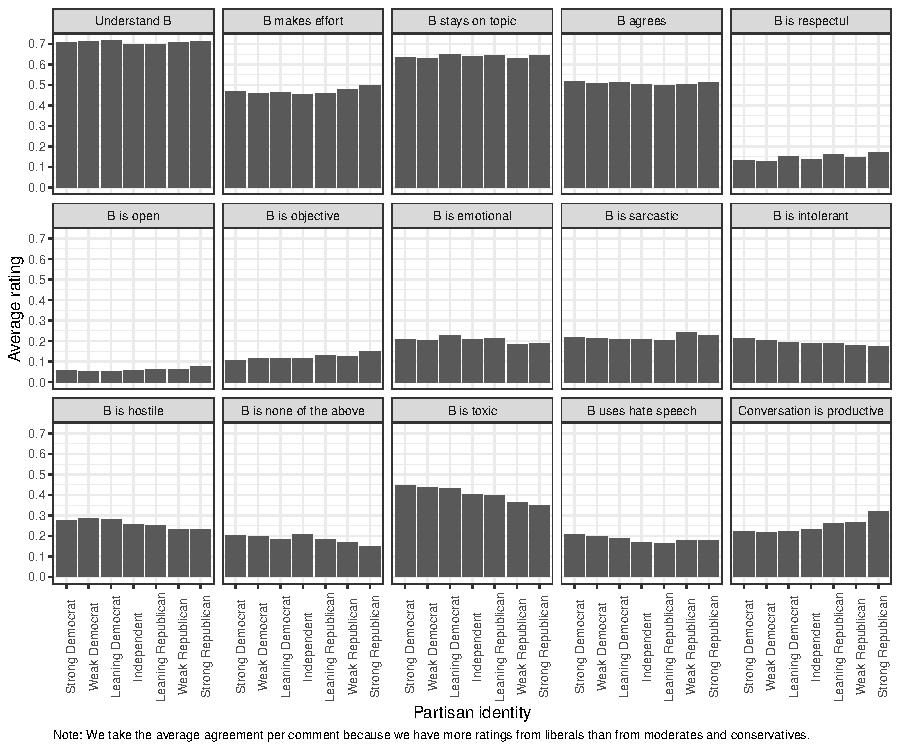
\includegraphics[width=1\linewidth]{figures/2_AvgAgreement_Partisanship.pdf}
    \caption{Variables measuring dimensions of civility by partisanship}
    \label{fig:civility-partisanship}
    \vspace{0.25cm}
    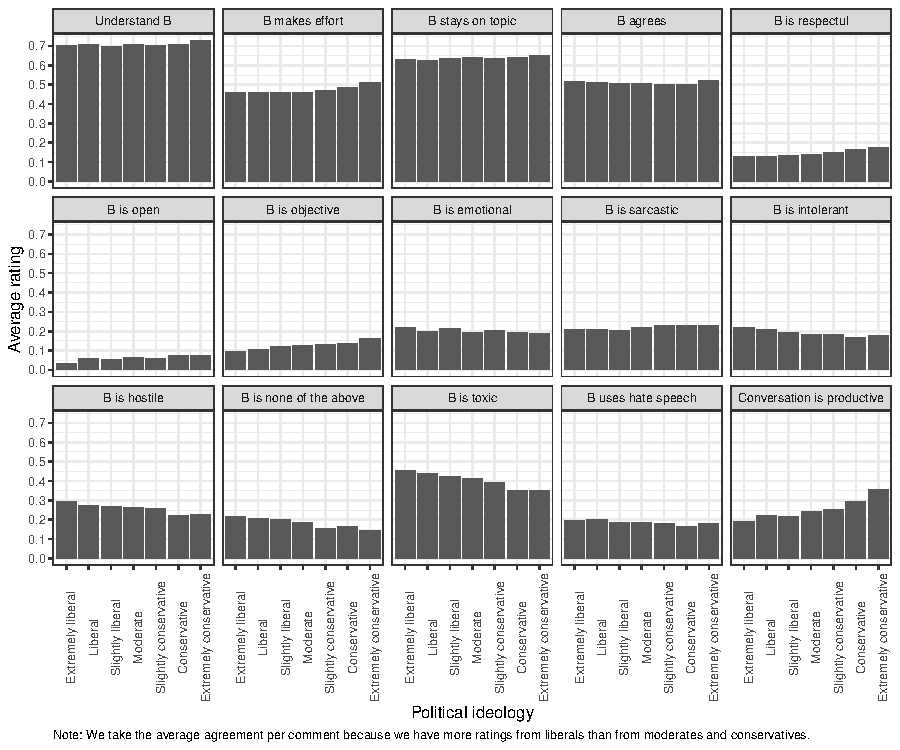
\includegraphics[width=1\linewidth]{figures/2_AvgAgreement_Ideo.pdf}
    \caption{Variables measuring dimensions of civility by political ideology}
    \label{fig:civility-ideology}
\end{figure}

%%%%%%%%%%%%%%%%%%%%%%%%%%%%%%%%%%%%%%%%%%
% Tables % 
\renewcommand{\arraystretch}{0.9}
\begin{table}[!h]
\centering
\caption{\label{tab:summ-tab1}Summary statistics on characteristics of survey respondents}
\centering
\begin{tabular}[t]{l|l|r|r|r|r|r|r}
\hline
Type & Variable & Min & Q25 & Mean & Median & Q75 & Max\\
\hline
 & BToxicNum & -1.00 & -1.00 & 0.25 & 0.00 & 1.00 & 2.00\\
\cline{2-8}
\multirow{-2}{*}{\raggedright\arraybackslash Dependent Variable} & BToxicNum01 & -0.42 & -0.42 & 0.00 & -0.08 & 0.25 & 0.58\\
\cline{1-8}
 & EducationNum & 1.00 & 3.00 & 3.05 & 3.00 & 3.00 & 5.00\\
\cline{2-8}
 & GenderMan & 0.00 & 0.00 & 0.49 & 0.00 & 1.00 & 1.00\\
\cline{2-8}
 & GenderOther & 0.00 & 0.00 & 0.02 & 0.00 & 0.00 & 1.00\\
\cline{2-8}
 & GenderWoman & 0.00 & 0.00 & 0.48 & 0.00 & 1.00 & 1.00\\
\cline{2-8}
 & Income2Sd & -0.58 & -0.30 & 0.00 & -0.13 & 0.38 & 1.79\\
\cline{2-8}
\multirow{-6}{*}{\raggedright\arraybackslash Demographics} & PolIdComp & 1.00 & 1.50 & 3.18 & 3.00 & 4.50 & 7.00\\
\hline
\end{tabular}
\end{table}


\begin{table}[!h]
\centering
\caption{\label{tab:summ-tab2}Summary statistics on conversation characteristics}
\centering
\begin{tabular}[t]{l|l|r|r|r|r|r|r}
\hline
Type & Variable & Min & Q25 & Mean & Median & Q75 & Max\\
\hline
 & antiabortion & 0.00 & 0.00 & 0.01 & 0.00 & 0.00 & 1.00\\
\cline{2-8}
 & antiamerica & 0.00 & 0.00 & 0.15 & 0.00 & 0.00 & 1.00\\
\cline{2-8}
 & antichristianity & 0.00 & 0.00 & 0.01 & 0.00 & 0.00 & 1.00\\
\cline{2-8}
 & anticlinton & 0.00 & 0.00 & 0.13 & 0.00 & 0.00 & 1.00\\
\cline{2-8}
 & antigun & 0.00 & 0.00 & 0.01 & 0.00 & 0.00 & 1.00\\
\cline{2-8}
 & antiimmigrant & 0.00 & 0.00 & 0.12 & 0.00 & 0.00 & 1.00\\
\cline{2-8}
 & antitrump & 0.00 & 0.00 & 0.12 & 0.00 & 0.00 & 1.00\\
\cline{2-8}
 & drugs & 0.00 & 0.00 & 0.02 & 0.00 & 0.00 & 1.00\\
\cline{2-8}
 & proabortion & 0.00 & 0.00 & 0.01 & 0.00 & 0.00 & 1.00\\
\cline{2-8}
 & proclinton & 0.00 & 0.00 & 0.02 & 0.00 & 0.00 & 1.00\\
\cline{2-8}
 & progun & 0.00 & 0.00 & 0.01 & 0.00 & 0.00 & 1.00\\
\cline{2-8}
 & proimmigrant & 0.00 & 0.00 & 0.01 & 0.00 & 0.00 & 1.00\\
\cline{2-8}
 & protrump & 0.00 & 0.00 & 0.06 & 0.00 & 0.00 & 1.00\\
\cline{2-8}
\multirow{-14}{*}{\raggedright\arraybackslash Topic} & suggestive & 0.00 & 0.00 & 0.13 & 0.00 & 0.00 & 1.00\\
\cline{1-8}
 & Emoji & 0.00 & 0.00 & 0.03 & 0.00 & 0.00 & 6.22\\
\cline{2-8}
 & achieve & 0.00 & 0.00 & 0.21 & 0.00 & 0.00 & 4.62\\
\cline{2-8}
 & cogproc & 0.00 & 0.00 & 1.62 & 2.16 & 2.77 & 4.62\\
\cline{2-8}
 & comm & 0.00 & 0.00 & 0.28 & 0.00 & 0.00 & 4.62\\
\cline{2-8}
 & conflict & 0.00 & 0.00 & 0.18 & 0.00 & 0.00 & 4.62\\
\cline{2-8}
 & death & 0.00 & 0.00 & 0.10 & 0.00 & 0.00 & 3.93\\
\cline{2-8}
 & emo\_neg & 0.00 & 0.00 & 0.22 & 0.00 & 0.00 & 4.62\\
\cline{2-8}
 & emo\_pos & 0.00 & 0.00 & 0.20 & 0.00 & 0.00 & 4.62\\
\cline{2-8}
 & ethnicity & 0.00 & 0.00 & 0.25 & 0.00 & 0.00 & 4.62\\
\cline{2-8}
 & female & 0.00 & 0.00 & 1.04 & 0.00 & 2.40 & 4.62\\
\cline{2-8}
 & food & 0.00 & 0.00 & 0.08 & 0.00 & 0.00 & 4.21\\
\cline{2-8}
 & home & 0.00 & 0.00 & 0.07 & 0.00 & 0.00 & 3.93\\
\cline{2-8}
 & i & 0.00 & 0.00 & 0.42 & 0.00 & 0.00 & 4.62\\
\cline{2-8}
 & leisure & 0.00 & 0.00 & 0.07 & 0.00 & 0.00 & 4.62\\
\cline{2-8}
 & male & 0.00 & 0.00 & 0.28 & 0.00 & 0.00 & 4.62\\
\cline{2-8}
 & money & 0.00 & 0.00 & 0.15 & 0.00 & 0.00 & 3.93\\
\cline{2-8}
 & moral & 0.00 & 0.00 & 0.36 & 0.00 & 0.00 & 4.62\\
\cline{2-8}
 & polite & 0.00 & 0.00 & 0.12 & 0.00 & 0.00 & 4.62\\
\cline{2-8}
 & politic & 0.00 & 0.00 & 0.39 & 0.00 & 0.00 & 4.62\\
\cline{2-8}
 & power & 0.00 & 0.00 & 0.60 & 0.00 & 1.35 & 4.62\\
\cline{2-8}
 & prosocial & 0.00 & 0.00 & 0.15 & 0.00 & 0.00 & 4.62\\
\cline{2-8}
 & relig & 0.00 & 0.00 & 0.19 & 0.00 & 0.00 & 4.62\\
\cline{2-8}
 & sexual & 0.00 & 0.00 & 0.19 & 0.00 & 0.00 & 4.62\\
\cline{2-8}
 & shehe & 0.00 & 0.00 & 0.75 & 0.00 & 1.83 & 4.62\\
\cline{2-8}
 & substances & 0.00 & 0.00 & 0.01 & 0.00 & 0.00 & 3.93\\
\cline{2-8}
 & swear & 0.00 & 0.00 & 0.54 & 0.00 & 0.00 & 4.62\\
\cline{2-8}
 & tech & 0.00 & 0.00 & 0.19 & 0.00 & 0.00 & 4.62\\
\cline{2-8}
 & they & 0.00 & 0.00 & 0.35 & 0.00 & 0.00 & 3.93\\
\cline{2-8}
 & tone\_neg & 0.00 & 0.00 & 1.03 & 0.00 & 2.13 & 4.62\\
\cline{2-8}
 & tone\_pos & 0.00 & 0.00 & 0.62 & 0.00 & 1.30 & 4.62\\
\cline{2-8}
 & we & 0.00 & 0.00 & 0.23 & 0.00 & 0.00 & 3.93\\
\cline{2-8}
 & work & 0.00 & 0.00 & 0.23 & 0.00 & 0.00 & 3.93\\
\cline{2-8}
\multirow{-33}{*}{\raggedright\arraybackslash LIWC} & you & 0.00 & 0.00 & 0.52 & 0.00 & 0.00 & 4.62\\
\cline{1-8}
 & Order & -3.00 & -2.00 & 0.00 & 0.00 & 2.00 & 3.00\\
\cline{2-8}
 & ideo\_commenterB & -0.96 & -0.37 & 0.14 & 0.14 & 0.76 & 1.01\\
\cline{2-8}
\multirow{-3}{*}{\raggedright\arraybackslash Other} & target\_likes\_count & 0.00 & 0.00 & 0.53 & 0.00 & 0.69 & 7.18\\
\hline
\end{tabular}
\end{table}


\begin{table}[!h]
\centering
\caption{\label{tab:summ-tab3}Summary statistics on conversation characteristics (2). Table shows word counts in LIWC categories transformed with $\log(1+x)$.}
\centering
\begin{tabular}[t]{llrrrrrr}
\toprule
Type & Variable & Min & Q25 & Mean & Median & Q75 & Max\\
\midrule
 & tone\_pos & 0 & 0 & 0.62 & 0.00 & 1.30 & 4.62\\
\cmidrule{2-8}
 & tone\_neg & 0 & 0 & 1.03 & 0.00 & 2.13 & 4.62\\
\cmidrule{2-8}
 & emo\_pos & 0 & 0 & 0.20 & 0.00 & 0.00 & 4.62\\
\cmidrule{2-8}
 & emo\_neg & 0 & 0 & 0.22 & 0.00 & 0.00 & 4.62\\
\cmidrule{2-8}
 & swear & 0 & 0 & 0.54 & 0.00 & 0.00 & 4.62\\
\cmidrule{2-8}
 & conflict & 0 & 0 & 0.18 & 0.00 & 0.00 & 4.62\\
\cmidrule{2-8}
 & prosocial & 0 & 0 & 0.15 & 0.00 & 0.00 & 4.62\\
\cmidrule{2-8}
 & polite & 0 & 0 & 0.12 & 0.00 & 0.00 & 4.62\\
\cmidrule{2-8}
 & moral & 0 & 0 & 0.36 & 0.00 & 0.00 & 4.62\\
\cmidrule{2-8}
 & comm & 0 & 0 & 0.28 & 0.00 & 0.00 & 4.62\\
\cmidrule{2-8}
 & cogproc & 0 & 0 & 1.62 & 2.16 & 2.77 & 4.62\\
\cmidrule{2-8}
 & politic & 0 & 0 & 0.39 & 0.00 & 0.00 & 4.62\\
\cmidrule{2-8}
 & ethnicity & 0 & 0 & 0.25 & 0.00 & 0.00 & 4.62\\
\cmidrule{2-8}
 & tech & 0 & 0 & 0.19 & 0.00 & 0.00 & 4.62\\
\cmidrule{2-8}
 & leisure & 0 & 0 & 0.07 & 0.00 & 0.00 & 4.62\\
\cmidrule{2-8}
 & home & 0 & 0 & 0.07 & 0.00 & 0.00 & 3.93\\
\cmidrule{2-8}
 & work & 0 & 0 & 0.23 & 0.00 & 0.00 & 3.93\\
\cmidrule{2-8}
 & money & 0 & 0 & 0.15 & 0.00 & 0.00 & 3.93\\
\cmidrule{2-8}
 & relig & 0 & 0 & 0.19 & 0.00 & 0.00 & 4.62\\
\cmidrule{2-8}
 & substances & 0 & 0 & 0.01 & 0.00 & 0.00 & 3.93\\
\cmidrule{2-8}
 & sexual & 0 & 0 & 0.19 & 0.00 & 0.00 & 4.62\\
\cmidrule{2-8}
 & food & 0 & 0 & 0.08 & 0.00 & 0.00 & 4.21\\
\cmidrule{2-8}
 & death & 0 & 0 & 0.10 & 0.00 & 0.00 & 3.93\\
\cmidrule{2-8}
 & male & 0 & 0 & 0.28 & 0.00 & 0.00 & 4.62\\
\cmidrule{2-8}
 & female & 0 & 0 & 1.04 & 0.00 & 2.40 & 4.62\\
\cmidrule{2-8}
 & shehe & 0 & 0 & 0.75 & 0.00 & 1.83 & 4.62\\
\cmidrule{2-8}
 & they & 0 & 0 & 0.35 & 0.00 & 0.00 & 3.93\\
\cmidrule{2-8}
 & you & 0 & 0 & 0.52 & 0.00 & 0.00 & 4.62\\
\cmidrule{2-8}
 & i & 0 & 0 & 0.42 & 0.00 & 0.00 & 4.62\\
\cmidrule{2-8}
 & we & 0 & 0 & 0.23 & 0.00 & 0.00 & 3.93\\
\cmidrule{2-8}
 & Emoji & 0 & 0 & 0.03 & 0.00 & 0.00 & 6.22\\
\cmidrule{2-8}
 & power & 0 & 0 & 0.60 & 0.00 & 1.35 & 4.62\\
\cmidrule{2-8}
\multirow{-33}{*}{\raggedright\arraybackslash LIWC} & achieve & 0 & 0 & 0.21 & 0.00 & 0.00 & 4.62\\
\bottomrule
\end{tabular}
\end{table}

\clearpage
% End tables 
%%%%%%%%%%%%%%%%%%%%%%%%%%%%%%%%%%%%%%%%%%%%

% Regression table 
\clearpage
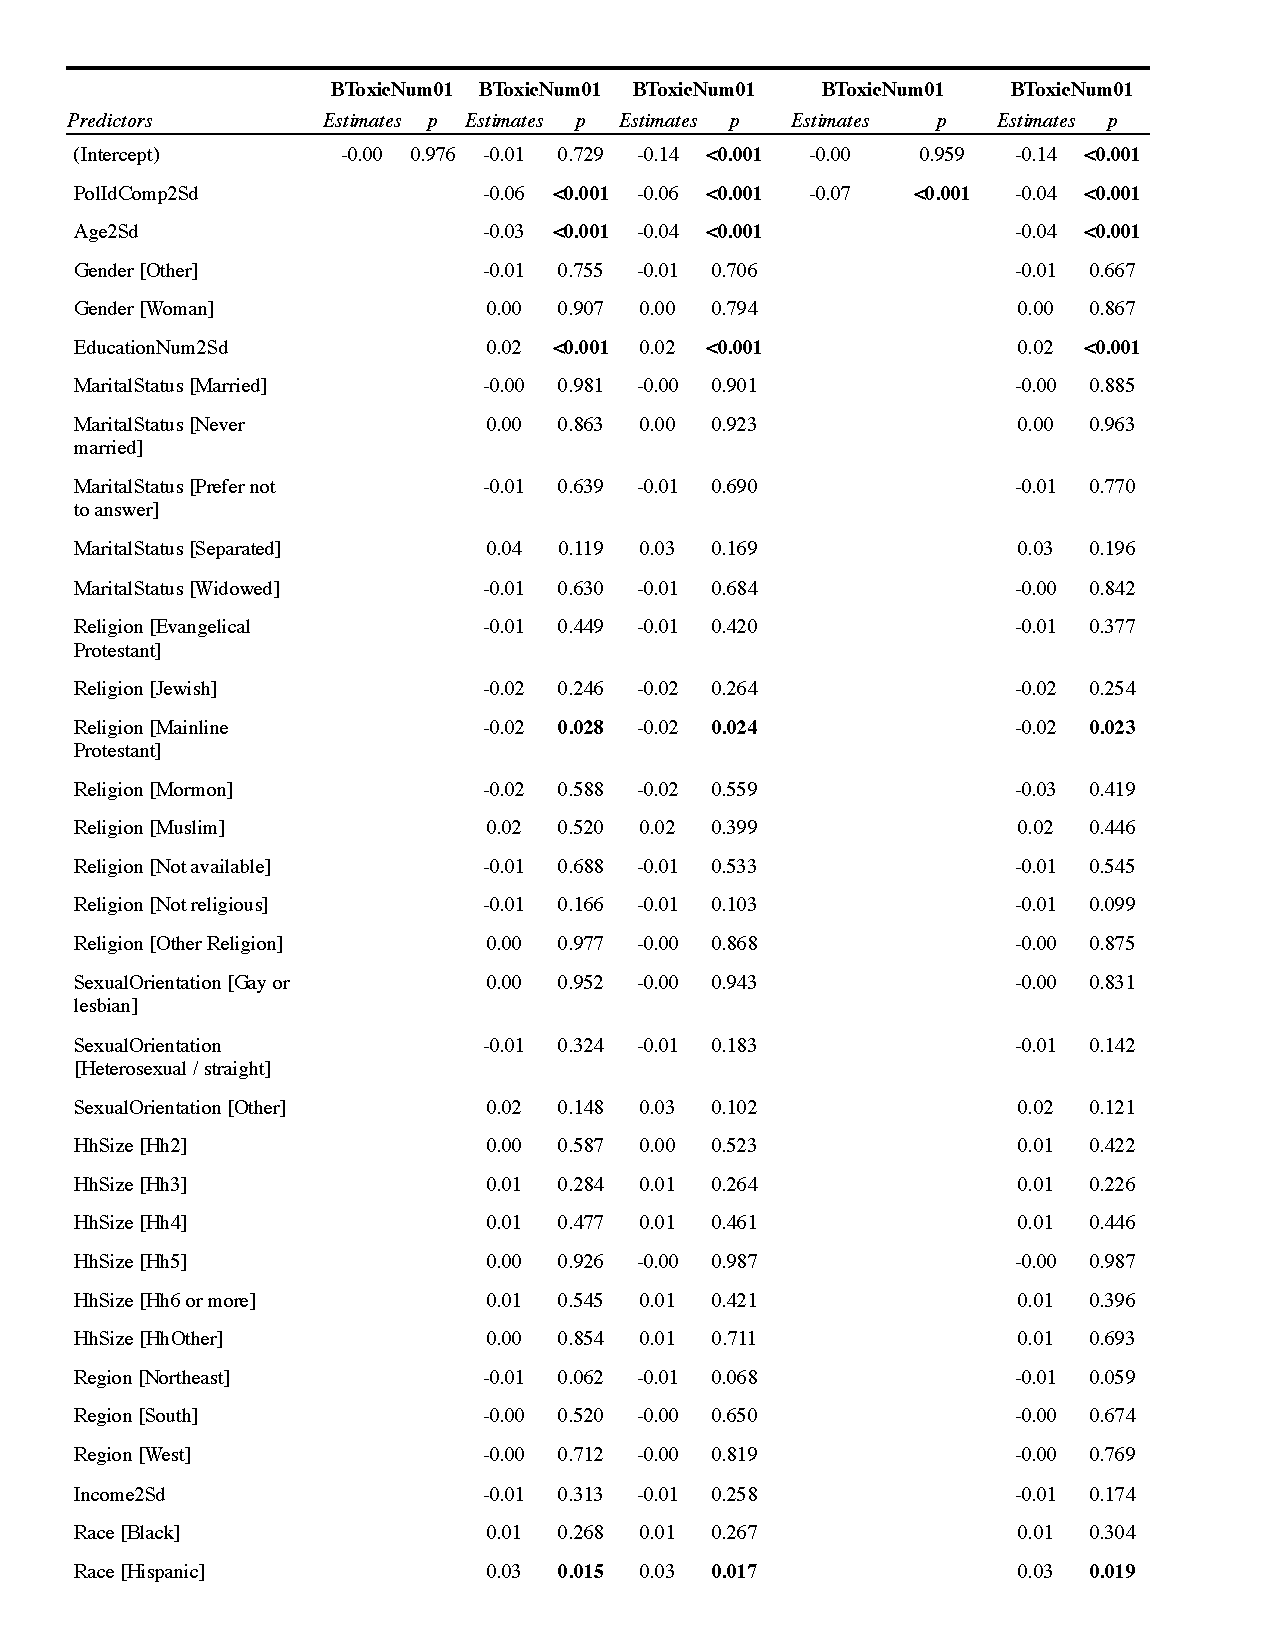
\includepdf[pages={1-},scale=0.95]{tox.html.pdf}
\end{document}
